%%%%%%%%%%%%%%%%%%%%%%%%%%%%%%%%%%%%%%%%%%%%%%%%%%%%%%%%%%%%%%%%%%%%%%%%%%%%%%%%
% $Id: latex.tex 112 2015-10-06 14:31:36Z klugeflo $
%%%%%%%%%%%%%%%%%%%%%%%%%%%%%%%%%%%%%%%%%%%%%%%%%%%%%%%%%%%%%%%%%%%%%%%%%%%%%%%%

\chapter{Short Introduction to \LaTeX}
\label{c:latex}

%%%%%%%%%%%%%%%%%%%%%%%%%%%%%%%%%%%%%%%%%%%%%%%%%%%%%%%%%%%%%%%%%%%%%%%%%%%%%%%%

%%%%%%%%%%%%%%%%%%%%%%%%%%%%%%%%%%%%%%%%%%%%%%%%%%%%%%%%%%%%%%%%%%%%%%%%%%%%%%%%
%%%%%%%%%%%%%%%%%%%%%%%%%%%%%%%%%%%%%%%%%%%%%%%%%%%%%%%%%%%%%%%%%%%%%%%%%%%%%%%%

\section{Table of Contents}

%%%%%%%%%%%%%%%%%%%%%%%%%%%%%%%%%%%%%%%%%%%%%%%%%%%%%%%%%%%%%%%%%%%%%%%%%%%%%%%%

Organize your work by using chapters
(\verb+\chapter+), sections (\verb+\section+), and subsections
(\verb+\subsection+ and \verb+\subsubsection+). If these are not
sufficient, you can also use paragraphs (\verb+\paragraph+).
In the template provided here, up to the the outline level \texttt{subsection}
the outline numbers are numbers are automatically generated and the corresponding
entries end up in the table of contents. If you do not want this at certain places
use the * form of the command.

%%%%%%%%%%%%%%%%%%%%%%%%%%%%%%%%%%%%%%%%%%%%%%%%%%%%%%%%%%%%%%%%%%%%%%%%%%%%%%%%
%%%%%%%%%%%%%%%%%%%%%%%%%%%%%%%%%%%%%%%%%%%%%%%%%%%%%%%%%%%%%%%%%%%%%%%%%%%%%%%%

\section{Text Composition}

%%%%%%%%%%%%%%%%%%%%%%%%%%%%%%%%%%%%%%%%%%%%%%%%%%%%%%%%%%%%%%%%%%%%%%%%%%%%%%%%

\LaTeX~offers several ways to structure a text.
The following sections explain the use of bullets, tables, and images.

%%%%%%%%%%%%%%%%%%%%%%%%%%%%%%%%%%%%%%%%%%%%%%%%%%%%%%%%%%%%%%%%%%%%%%%%%%%%%%%%

\subsection{Lists}

\LaTeX~has three kinds of lists. Probably the most widely used is the \texttt{itemize} environment:
\begin{itemize}
\item This is the first bullet point.
\item Another bullet point.
\item Lists can consist of longer or multiline texts. \LaTeX~ takes care of the current layout
the same way as for normal text.
\end{itemize}

For enumerated lists the \texttt{enumerate} environment can be used:
\begin{enumerate}
\item Single bullet points are only set with \verb+\item+.
\item The enumeration will be generated automatically by \LaTeX~.
\item Lists can be nested:
  \begin{itemize}
  \item Here with an unnumbered list.
  \end{itemize}
\end{enumerate}

If you want to explain multiple terms the \texttt{description}-environment can be used:
\begin{description}
\item[Usage] Descriptions are set like all other enumerations, with the term being describe
in brackets right after \verb+\item+.
\item[Text markup] You can highlight text with
  \verb+\textXX+ in \textbf{bold}, \textit{cursive} or
  \textsc{small caps}. For simple highlighting, you can use the \verb+\emph+ command.
\item[Document class] The first command of a \LaTeX-Dokuments defines the document class, i.e.,
  the template. For example, this document, uses the class \texttt{sikthesis}\\
  (\verb+\documentclass{sikthesis}+). You can pass the document class
  an optional argument \verb+[draft]+ to create a draft of the document (this will compile
  much faster, which can be useful during writing). 
  Images are then displayed only as empty frames, 
  and \LaTeX~ marks issues in the margin, e.g., if there are still
  problems with pagination or overlong text. These
  problems can generally be solved by slightly rewording the text.
\end{description}

%%%%%%%%%%%%%%%%%%%%%%%%%%%%%%%%%%%%%%%%%%%%%%%%%%%%%%%%%%%%%%%%%%%%%%%%%%%%%%%%

\subsection{Tables}

A table can be generated in \LaTeX~using the \texttt{tabular} environment:

\begin{tabular}{|l|r|p{3cm}|}
\hline
Row 1 & 2nd cell & long text that is automatically wrapped\\\hline
Row 2 & 2nd cell & short text\\\hline
\end{tabular}

Tables can also be embedded in \texttt{table} environments.
\LaTeX~then places these tables \emph{floatingly}.
Such tables can then also be provided with a \verb+\caption+ and
referenced in the text (see the \ref{t:example} table).
If the \verb+\caption+ text is very long, it is recommended to add a short text to the
macro for the table listing as an optional argument.\\
\verb+\caption[Text for table listing]{Caption}+.

\begin{table}[hbtp]
\centering
\begin{tabular}{|l|r|p{3cm}|}
  \hline
  Row 1 & 2nd cell & long text that is automatically wrapped\\\hline
  Row 2 & 2nd cell & short text\\\hline
  \end{tabular}
\caption[Example for a floating table]{Example for a floating table.
Always provide an informative caption.}
\label{t:example}
\end{table}

%%%%%%%%%%%%%%%%%%%%%%%%%%%%%%%%%%%%%%%%%%%%%%%%%%%%%%%%%%%%%%%%%%%%%%%%%%%%%%%%

\subsection{Figures}

As with tables, graphics should be placed in a flowing manner, so that
\LaTeX~takes care of their placement as much as possible. Figure
\ref{f:example} shows an example of such an image.

\begin{figure}[htbp]
  \centering
  
\includegraphics[width=0.6\textwidth]{uniwappen}
  \caption[Short description listoffigures]{Example for a figure, 
    60\% text width, the width can be configured as well, e.g., 6cm.}
  \label{f:example}
\end{figure}

If possible, use the \tikz~package to create diagrams.
Specify the description of the graphic directly in the \TeX~code.
This ensures in particular that captions in the graphic have the same
typeface as the text of your work.
An example of such a figure can be found in the
figures~\ref{f:tikz1} and \ref{f:tikz2}.
These figures also show how to create two graphics using
\verb+minipage+ environments side by side.
Another useful environment to achieve this is \verb+subfigure+.

\begin{figure}[htbp]
  \begin{minipage}{0.5\textwidth}
    \centering
    \begin{tikzpicture}[initial text={}]
      \node [state,initial] (start) {Start};
      \node [state,above right=of start] (s1) {S1};
      \node [state,below right=of start] (s2) {S2};
      \path [->]
      (start) edge (s1)
      (start) edge (s2)
      (s1) edge (s2)
      (s2) edge [loop right] node [right] {Endlosschleife} ();
    \end{tikzpicture}
    \caption{\tikz figure 1}
    \label{f:tikz1}
  \end{minipage}
  %
  \begin{minipage}{0.5\textwidth}
    \centering
    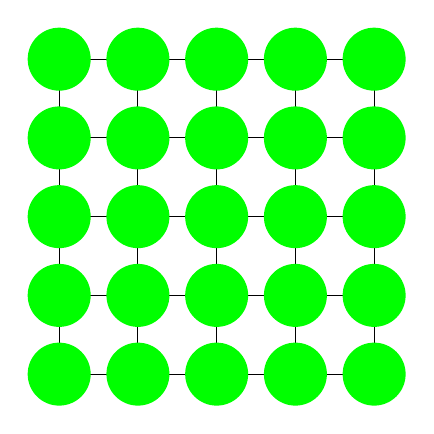
\begin{tikzpicture}
      \draw (0,0) grid (4,4);
      \foreach \x in {0,1,...,4} {
        \foreach \y in {0,1,...,4} {
          \fill [green] (\x,\y) circle (0.4cm);
        }
      }
    \end{tikzpicture}
    \caption{\tikz figure 2}
    \label{f:tikz2}
  \end{minipage}
\end{figure}

To create diagrams you can use the \verb+pgfplots+ package,
which is based on \tikz and PGF.
For examples see the figures~\ref{f:pgf1} and \ref{f:pgf2}.

\begin{figure}[htbp]
  \begin{minipage}{0.5\textwidth}
    \centering
    \begin{tikzpicture}
      \begin{axis}[
          width=0.8\textwidth,
          %ybar,
          %bar width=0.1cm,
          ylabel={Execution time (cycles)},
          xlabel={Core},
          legend style={at={(0.5,1.05)},anchor=south,legend
            columns=-1}
        ]
        
        %fullimg
        \addplot +[only marks,mark=+] coordinates {
          (0,770865)
          (1,329608)
          (2,550254)
          (3,770900)
        };
        
        %nokrep
        \addplot +[only marks,mark=x] coordinates {
          (0,693448)
          (1,369585)
          (2,531878)
          (3,694171)
        };
        
        %mossca
        \addplot +[only marks,mark=*] coordinates {
          (0,686010)
          (1,361362)
          (2,523655)
          (3,685948)
        };
        
        \legend{FI,SI,SD}
      \end{axis}
    \end{tikzpicture}
    
    \caption{pgf diagram 1}
    \label{f:pgf1}
  \end{minipage}
  %
  \begin{minipage}{0.5\textwidth}
    \centering
    
    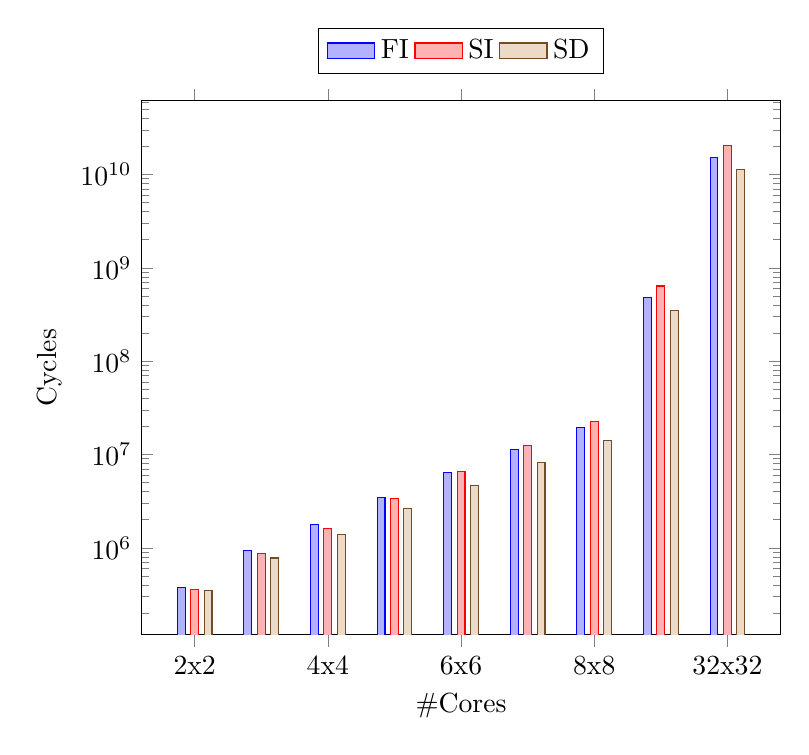
\begin{tikzpicture}
      \begin{semilogyaxis}[
          width=0.8\textwidth,
          ybar,
          bar width=0.1cm,
          ylabel={Cycles},
          xlabel={\#Cores},
          legend style={at={(0.5,1.05)},anchor=south,legend
            columns=-1},
          symbolic x coords={2x2,3x3,4x4,5x5,6x6,7x7,8x8,16x16,32x32}
        ]
        
        %fullimg
        \addplot +[area legend] coordinates {
          (2x2, 376662) (3x3, 946144) (4x4, 1794265) (5x5, 3470767) (6x6, 6352207) (7x7, 11348627) (8x8, 19489997) (16x16, 481008057) (32x32, 15336870167)
        };
        %nokrep
        \addplot +[area legend] coordinates {
          (2x2, 360174) (3x3, 861960) (4x4, 1628092) (5x5, 3382747) (6x6, 6623068) (7x7, 12603816) (8x8, 22750681) (16x16, 637517992) (32x32, 20568322109)
        };
        %mossca
        \addplot +[area legend] coordinates {
          (2x2, 349798) (3x3, 778817) (4x4, 1402881) (5x5, 2609504) (6x6, 4655134) (7x7, 8225318) (8x8, 14110261) (16x16, 349710481) (32x32, 11253110760)
        };
        \legend{FI,SI,SD}
      \end{semilogyaxis}
    \end{tikzpicture}
    \caption{pgf diagram 2}
    \label{f:pgf2}
  \end{minipage}
\end{figure}

%%%%%%%%%%%%%%%%%%%%%%%%%%%%%%%%%%%%%%%%%%%%%%%%%%%%%%%%%%%%%%%%%%%%%%%%%%%%%%%%
%%%%%%%%%%%%%%%%%%%%%%%%%%%%%%%%%%%%%%%%%%%%%%%%%%%%%%%%%%%%%%%%%%%%%%%%%%%%%%%%

\section{Mathematical Symbols}

%%%%%%%%%%%%%%%%%%%%%%%%%%%%%%%%%%%%%%%%%%%%%%%%%%%%%%%%%%%%%%%%%%%%%%%%%%%%%%%%

Mathematical formulas in texts are marked by \$ signs, e.g. $E=mc^2$.
Separate formulas are set in the following way:
\[f(x) = \frac{1}{\sigma\sqrt{2\pi}}
\exp\left(-\frac{(x-\mu)^2}{2\sigma^2}\right)\]
If you want to enumerate formulas use the \texttt{equation} environment:
\begin{equation}
  \label{eq:nd}
F(x) = \frac{1}{\sigma\sqrt{2\pi}} \int_{-\infty}^x
\exp\left(-\frac{(t-\mu)^2}{2\sigma^2}\right)\,dt
\end{equation}
The formula can now be referenced in the text using \verb+\eqref+:
Equation~\eqref{eq:nd}.

Please note that in mathematical mode, \LaTeX~regards each character as own variable.
The character string $size$ is therefore set as the product of the variables $s$, $i$,
$z$ and $e$ (the multiplication sign is usually not specified).
If you want to use a variable with a longer name instead, 
set this with \verb+\mathit{...}+, e.g. $\mathit{size}$.
If you look closely, you will see that in this case the
character spacing is set differently.

%%%%%%%%%%%%%%%%%%%%%%%%%%%%%%%%%%%%%%%%%%%%%%%%%%%%%%%%%%%%%%%%%%%%%%%%%%%%%%%%
%%%%%%%%%%%%%%%%%%%%%%%%%%%%%%%%%%%%%%%%%%%%%%%%%%%%%%%%%%%%%%%%%%%%%%%%%%%%%%%%

\section{External References}

%%%%%%%%%%%%%%%%%%%%%%%%%%%%%%%%%%%%%%%%%%%%%%%%%%%%%%%%%%%%%%%%%%%%%%%%%%%%%%%%

Literature references are managed using BibTeX. For this purpose the
references are stored in a file of their own (e.g. \texttt{thesis.bib})
and provided with abbreviations. These can then be referenced in the text.
Note that you now have to \enquote{translate} your document twice.
Between the two \texttt{latex} -or \texttt{pdflatex} calls you must call 
\texttt{bibtex}. More information on this and on using
\LaTeX~ in general can be found in \cite{kopka} and online.

Here is an example for an internet reference \cite{heise} and one for a
reference with multiple authors \cite{liu73acm}.

%%%%%%%%%%%%%%%%%%%%%%%%%%%%%%%%%%%%%%%%%%%%%%%%%%%%%%%%%%%%%%%%%%%%%%%%%%%%%%%%
%%%%%%%%%%%%%%%%%%%%%%%%%%%%%%%%%%%%%%%%%%%%%%%%%%%%%%%%%%%%%%%%%%%%%%%%%%%%%%%%

\section{Helpers}

%%%%%%%%%%%%%%%%%%%%%%%%%%%%%%%%%%%%%%%%%%%%%%%%%%%%%%%%%%%%%%%%%%%%%%%%%%%%%%%%

The following packages are a great help when working with \LaTeX to write your thesis:
\begin{description}
\item[acro] allows you to conveniently use abbreviations without having to track them yourself.
  You do not have to keep track whether they have already been used in a particular place.
  Using \verb+\DeclareAcronym{id}{short=...,long=...}+ in the document preamble, you can define the
  acronyms. In the text the acronym is then used by means of \verb+\ac{id}+.
  The first time it is used, the long name is generated, as for example in \enquote{\ac{os},}
  for later use only the the abbreviation is output, e.g., \enquote{\ac{os}.}\todo{Yes, the quotes
  are set correctly in English like this. :)}
  You can generate a list of all existing acronyms with \verb+\printacronyms+.
\item[todonotes] are helpful for the ongoing work on the document.
  They can be used to create marginal notes, e.g., for later editing.
  \todo{Example todo note}
  This package can also be used to create placeholder graphics like the one in
  Figure ~\ref{f:example}.
  Using \verb+\todototoc+ you can get a list of all existing todo notes.
\end{description}

%%%%%%%%%%%%%%%%%%%%%%%%%%%%%%%%%%%%%%%%%%%%%%%%%%%%%%%%%%%%%%%%%%%%%%%%%%%%%%%%
%%% Local Variables: 
%%% mode: latex
%%% TeX-master: thesis
%%% TeX-PDF-mode: t
%%% End: 
%%%%%%%%%%%%%%%%%%%%%%%%%%%%%%%%%%%%%%%%%%%%%%%%%%%%%%%%%%%%%%%%%%%%%%%%%%%%%%%%
%<!-- Local IspellDict: en -->
